%%%%%%%%%%%%%%%%%%%%%%%%%%%%%%%%%%%%%%%%%%%%%%%%
% 4: Diseño y resolución del trabajo realizado
%%%%%%%%%%%%%%%%%%%%%%%%%%%%%%%%%%%%%%%%%%%%%%%%
\chapter{Diseño y resolución del trabajo realizado}
\label{diseno}

Después de estudiar cual es la situación actual de la enseñanza de la programación a un nivel global y los diferentes proyectos que promueven el \emph{pensamiento computacional}, en este capítulo se analizarán cuales son las necesidades del proyecto Robode y como se han resuelto.

Como ya se ha mencionado anteriormente, se creará un simulador de un robot, al que hemos denominado \emph{Robode}, y se integrará en la plataforma Descubre la programación. Robode  estará dentro de un mundo del que podrá moverse con libertad y con el que podrá interactuar. El robot tendrá dos ruedas que se mueven independientemente (con un motor para cada una de ellas) y dispondrá de sensores que informarán de posibles colisiones con obstáculos. También, el robot tendrá la capacidad de detectar líneas o caminos pintados en el suelo, sabiendo también en que dirección detecta (o no) la linea.

Adicionalmente, el robot y el mundo en el que este se encuentra será dibujado en un elemento \emph{canvas} de HTML5, al igual que ocurre en la plataforma Descubre.


Como se puede ver, Robode es la unión de varios de los proyectos que se han analizado en el capítulo \ref{estado-arte}. Por una parte, la idea principal de crear un simulador es igual a la que se ha realizado en Robomind (el cual se analiza en la sección \ref{sec:robomind}) pero simulando un robot en un mundo continuo y con características similares a las de Moway (analizado en la sección \ref{sec:moway}). Por último, se ejecutará en un entorno web, como bien puede ser el ejemplo de las herramientas que proporcionan CodeHS (sección \ref{sec:CodeHS}) y Code.org (sección \ref{sec:Code.org}). 


En las secciones siguientes se va a estudiar como se ha diseñado y creado Robode, que características tiene y cual ha sido la implementación exacta llevada a cabo.



\section{Motor físico}
\label{sec:motor-fisico}

El simulador representará un mundo con un robot y una serie de obstáculos que interfieren entre ellos. Los obstáculos podrán colisionar entre ellos o con el robot. También será necesario simular lineas en el suelo y la detección de las mismas. Todo ello con un paso del tiempo realista. Para ello, es necesario utilizar un motor físico que simule la creación de cuerpos en el mundo, su movimiento por el mismo y el contacto entre ellos, generando una reacción similar a la producida en el mundo real.

Para la creación del mundo y de las físicas que gestionan las colisiones y la interacción entre todos los elementos del simulador se han estudiado dos motores físicos: PhysicsJS\footnote{Página oficial de la librería PhysicsJS (\url{http://wellcaffeinated.net/PhysicsJS}).} y Box2D\footnote{El manual de uso de Box2D se puede encontrar en \cite{box2d-manual}. La documentación del proyecto se puede encontrar en (\url{http://www.box2dflash.org/docs/2.1a/reference/}).} \cite{box2d}. Dos librerías muy versátiles y de software libre que trabajan sobre entornos web.

PhysicsJS  es una librería escrita enteramente en Javascript por Jasper Palfree que aún está en fase beta. Por otra parte, Box2D es una famosa librería implementada originalmente para Flash\footnote{Página oficial de la librería Box2D para Flash (\url{http://www.box2dflash.org}).} con una gran comunidad de programadores utilizando dicha librería, lo cual siempre es de ayuda para resolver dudas y solucionar problemas. 

Box2D ha sido portada a Javascript dos veces. Una de ellas por Yayushi Ando y se llama Box2Djs\footnote{Página oficial de Box2Djs (\url{http://box2d-js.sourceforge.net}).} pero el proyecto no ha sido continuado y está desactualizado. El otro intento de llevar Box2D a Javascript ha culminado en Box2Dweb\footnote{El repositorio de Box2Dweb está alojado en GitHub (\url{https://github.com/hecht-software/box2dweb}).}. Como se puede leer en \cite[capítulo 13]{box2d-manual}, Box2D usa una serie de aproximaciones para representar las colisiones de manera eficiente. Principalmente, son dos las limitaciones que podría afectar al simulador del robot: (a) existe un desliz de aproximadamente 0.5 cm entre la forma que tiene un cuerpo y la colisión del mismo y (b) Box2D no maneja correctamente los cuerpos cóncavos. 

Al final, se ha establecido que la librería a utilizar será Box2Dweb. En cuanto a las limitaciones que puedan afectar a Robode, estas no son un gran problema a la solución del simulador puesto que: el desliz producido en limitación (a) es muy pequeño y en el caso del simulador, impercetible. Con respecto a la limitación (b), en el caso de que se quiera construir cuerpos cóncavos, se puede solucionar creando más de un cuerpo convexo que cree una forma \emph{global} cóncava.

Una vez que se ha aclarado que la librería utilizada es \texttt{Box2Dweb}, por simplicidad, a partir de ahora nos referiremos a ésta simplemente como \texttt{Box2D}.

\subsection{Definición del Mundo}
\label{sec:definicion-mundo}

En \texttt{Box2D} existen una serie de objetos que representan al mundo y los diferentes elementos que lo componen.  Estos son: el Mundo (World), los Cuerpos (Bodies), los Accesorios (Fixtures) y las Articulaciones o elementos constrictores (Joints).

El núcleo de Box2D es el objeto \emph{World}, el cual define los parámetros básicos que regirán la simulación más tarde, como puede ser el ratio de actualización o la gravedad. También crea y almacena el resto de objetos de Box2D, como los \emph{Bodies}, las \emph{Fixtures} y los \emph{Joints}, entre otros.

Para la creación de nuestro mundo, hemos decidido que tendrá una vista \emph{top-down}, es decir, una vista del mundo desde arriba, desde el cielo. De esta manera se consigue una vista superior de todo el circuito simplificando la comprensión del movimiento del robot sobre el circuito.

Una de las características más importantes de \texttt{Box2D} es la posibilidad de dotar a la aplicación que se está creando de un efecto gravitatorio de manera nativa al motor. Lo normal sería establecer éste valor con un vector de dirección hacia el suelo (hacia la parte baja de la pantalla) con la fuerza que se quiera simular. Esto provocaría que los cuerpos del mundo estuvieran constantemente sometidos a una fuerza que los mueve en dirección a ese vector, normalmente hacia el suelo.  

En el caso de Robode, al tener una vista superior del circuito, establecer una gravedad provocaría que el robot y el resto de cuerpos del circuito se movieran de forma anómala. Por esto, es necesario crear un mundo sin gravedad. En el listado del código \ref{code:world-gravedad} podemos ver como se ha establecido la gravedad del mundo a un vector con valor 0 en ambos ejes de coordenadas. 

\begin{lstlisting}[language={Javascript},label={code:world-gravedad}, caption={Definición del objeto \texttt{World} en Box2D con gravedad 0 y permitiendo que los cuerpos sean capaces de dormir.}]
Simulator.World = new b2World(
	new b2Vec2(0, 0), //gravity
	true //allow sleep
);
\end{lstlisting}

Otra característica importante en Box2D y que tiene un gran impacto en el rendimiento de la simulación es que los cuerpos puedan \emph{dormir}. Un cuerpo \emph{dormirá} cuando éste esté inactivo, es decir, cuando no esté siendo sometido a ninguna fuerza o sobre el se aplican fuerzas, pero éstas no son capaces de alterar su estado (posición, ángulo de giro, etc)\footnote{Esto ocurre generalmente cuando un objeto está sobre una superficie cuya forma y la del cuerpo hace que éste se mantenga quieto. Un ejemplo de esto puede ser un cuadrado sobre una superficie plana y horizontal con una gravedad hacia el suelo.}. En la línea 3 del listado de códigos \ref{code:world-gravedad} se puede ver como se ha establecido que los cuerpos del mundo sean capaces de dormir. Así, se consigue que el motor no simule los cuerpos que estén inactivos, mejorando el rendimiento de la aplicación.

Por último, queda definir el \emph{paso del tiempo} en Box2D. Para ello, es necesario ejecutar la función \texttt{Simulator.World.Step()} cada vez que queramos que se ejecute un \emph{paso} en nuestro mundo (esto es equivalente a un \emph{tic} de reloj). Esta función ordenará al motor que aplique todas las fuerzas necesarias sobre los cuerpos del mundo (gravedad, colisiones, deslizamientos, etc). Obviamente, es en este momento cuando se ejecutará la detección de colisiones por parte del motor de físicas. Justo después de ejecutar un paso se deben eliminar las fuerzas que afectan a los objetos para que se produzca un movimiento y efecto natural de las distintas fuerzas en los cuerpos. Esto se consigue con la función \texttt{Simulator.World.ClearForces()}.

En el listado del código  \ref{code:world-step} se puede ver con más detalle las funciones básicas que se deben ejecutar para que se produzca una actualización del mundo en Box2D.

\begin{lstlisting}[language={Javascript},label={code:world-step}, caption={Actualización del mundo en \texttt{Box2D}.}]
// (...)
Simulator.World.Step(
	1 / 60, //frame-rate
	10, //velocity iterations
	10 //position iterations
);

Simulator.World.ClearForces();

// (...)
\end{lstlisting}


\subsubsection{Creación de elementos en Box2D}


La creación de elementos (\emph{bodies}, \emph{fixtures}, \emph{joints}, etc) en Box2D utiliza un \emph{patrón factoría}, teniendo que definir primero en un objeto plantilla (definición) las características que tendrá el elemento a crear y luego diciéndole a \texttt{World} que cree dicho elemento a partir de la plantilla.

A continuación se explicarán las características principales de los elementos de Box2D y sus propiedades mas importantes.

\subsubsection*{Objeto \texttt{Body}}

Los cuerpos en Box2D pueden ser dinámicos (tipo \texttt{b2\_dynamicBody}) o estáticos (tipo \texttt{b2\_staticBody }). Un cuerpo dinámico podrá moverse y se verá afectado por el entorno y otros cuerpos. Un cuerpo estático será inmune a fuerzas como la gravedad y su posición no cambiará. Robode y todos sus componentes serán cuerpos dinámicos mientras que las fronteras del mundo, serán cuerpos estáticos. También, un cuerpo está activo si su propiedad \texttt{sleep} está activa. El efecto de un cuerpo inactivo ya se ha explicado en la sección \ref{sec:definicion-mundo}.

Un cuerpo conoce los \emph{fixtures} asociados a él (que puede ser más de uno) y los \emph{joints} a los que está atado.

Es el objeto \texttt{Body} el que contiene todas las propiedades físicas y que afectan al movimiento del mismo, como por ejemplo: la velocidad lineal y angular, el ángulo de rotación o la masa. Por supuesto, también la posición. Para obtener la posición de un cuerpo se utiliza el método \texttt{GetWorldCenter()} para obtener la posición en el mundo del centro de masas del cuerpo.


Las propiedades \texttt{linearDamping} y \texttt{angularDamping}\footnote{Aquí, con \emph{damping} se refiere al efecto de suelo mojado y el deslizamiento que un cuerpo tiene sobre una superficie, en especial cuando el cuerpo frena.} sirven para reducir la velocidad lineal y angular respectivamente cuando en el frenado.

%, y no con respecto al origen del mismo. Esto tiene que ver con las \emph{fixtures} que tenga asociadas dicho cuerpo. Por ejemplo, si un cuerpo tiene mas de una \emph{fixture}, la posición origen del cuerpo no representará la del 

 %ya que se puede definir la posición del cuerpo y la de la \emph{fixture} de manera que no coincidan. De esta manera, la función \texttt{GetWorldPosition()} obtendrá la posición correcta del cuerpo con respecto a la del \emph{fixture}.

Adicionalmente, se ha modificado el prototipo de las clases \texttt{b2Body} y \texttt{b2BodyDef} (clase plantilla para crear \emph{bodies}) para añadir una característica más al cuerpo, el nombre que se le asigna al cuerpo. Esto se usará principalmente para poder distinguir estos objetos fácilmente en una colisión.


\subsubsection*{Objeto \texttt{Fixture}}

Los objetos \texttt{b2Fixture} definen la apariencia del objeto al que están asociado y las características físicas que le harán interactuar con el mundo de una u otra manera.

Box2D proporciona dos clases principales para definir la forma de las \emph{fixtures}: \texttt{b2CircleShape()} y \texttt{b2PolygonShape()}. La primera representa a una forma circular y es necesario indicar el radio del circulo a crear. La segunda forma representa a un polígono. Los polígonos tienen dos formas principales de definirse:

\begin{itemize}
	\item Con forma de caja definiendo su ancho y largo (con el método \texttt{SetAsBox()}).
	\item Con una forma libre. Es necesario indicar los vértices del polígono y su cantidad (con el método \texttt{AsArray()}). Es así como se pueden crear triángulo o trapecios en Box2D, por ejemplo. En este caso es importante no crear formas cóncavas, pues provocarán errores en la simulación.
\end{itemize}


Además, un \emph{fixture} tiene propiedades de densidad, fricción y restitución que definirá la interacción de este con el mundo. La densidad es usada para calcular la masa del cuerpo al que está asociada la \emph{fixture}. La fricción se usa para hacer los cuerpos deslizarse de una manera realista. La restitución de un cuerpo es la elasticidad de este ante un impacto y según su valor, si rebota más o menos contra una superficie. 

Los valores de fricción y restitución oscilan entre 0 y 1. Siendo 0 la anulación de la propiedad y 1 el máximo valor que se le puede dar.


\subsubsection*{Objeto \texttt{Joint}}


Un \emph{Joint} es un elemento constrictor entre dos cuerpos, que controla el movimiento que hacen los cuerpos pegados por el joint. El punto por el que se une un cuerpo a un joint se denomina \emph{ancla}.

Hay distintos tipos de joints que limitan el movimiento de los cuerpos de diferentes maneras. A continuación se nombrarán los más importantes:

\begin{itemize}
	\item \texttt{Revolute} es un joint que fuerza a dos cuerpos a compartir el mismo \emph{ancla} con un cierto ángulo de libertad. También se puede configurar un \emph{motor} que hará girar el ancla y por tanto a los cuerpos.
	\item \texttt{Distance} es un joint que permite ata los cuerpos pero como si estuvieran sujetos a una cuerda. Los cuerpos tendrán una distancia máxima que se pueden separar (la longitud de la cuerda) pero no una mínima, pudiendo incluso chocar.
	\item \texttt{Prismatic} es un joint que simula el movimiento de un cuerpo unicamente sobre un eje de coordenadas, permitiendo movimientos como los de un ascensor.
\end{itemize}

En el simulador solo usaremos \emph{Joints} de tipo \emph{Revolute}, definidos por la clase \texttt{b2RevoluteJoint}.  En la inicialización del joint se deben indicar los dos cuerpos y el punto de ancla. También hay que establecer las propiedades relacionadas al motor (propiedad \texttt{enableMotor}), si se quiere que exista un límite de movimiento o no (propiedad \texttt{enableLimit}) y el valor máximo de torsión que se permite (propiedad \texttt{maxMotorTorque}).

\subsection{Construcción del robot}
\label{sec:contruccion-robot}

Para la creación del robot, un referente importante ha sido el robot de Moway. La forma y disposición de los sensores es similar a la simulada en Robode. Otro objetivo a cumplir era el de crear una simulación que imitara un comportamiento natural del robot a la hora de moverse, de chocar o de detenerse. Por tanto, se han establecido diferentes propiedades en los cuerpos para cumplir este objetivo.

Anteriormente ya se ha mencionado que el robot tendrá 2 ruedas, 2 sensores que detectarán líneas y otros 4 que detectaran colisiones. Todos estos elementos del robot están modelados en cuerpos separados. No obstante, es necesario que se mantengan unidos y se muevan a la vez.

En la figura \ref{fig:robot-skel} se puede ver un esqueleto del Robode.

\begin{figure}[!ht]
	\begin{centering}
		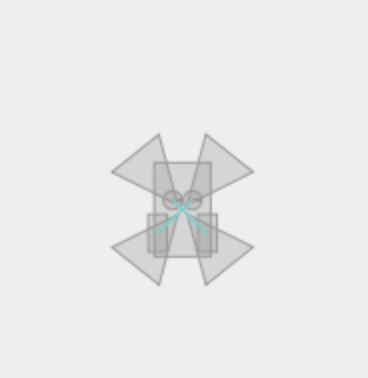
\includegraphics[width=0.5\textwidth]{images/robot-skel.png}
			\caption{Esqueleto del robot que muestra los diferentes \emph{bodies} y \emph{joints} que lo forman.}
				\label{fig:robot-skel}
	\end{centering}
\end{figure}

En las siguientes secciones se explicará más en detalle como se han creado cada una de las partes del robot.
 
\subsubsection*{Cuerpo principal}
\label{sec:cuerpo-principal}

El cuerpo principal está modelado como un rectángulo. Éste será más largo que ancho y tendrá el resto de cuerpos (sensores y ruedas) \emph{atados} a él con joints. El cuerpo principal de Robode será dinámico, así como los sensores y ruedas.

La forma se ha creado creando una fixture con forma poligonal. Se ha utilizado la función \texttt{SetAsBox()} que permite definir el ancho y alto del polígono, creándolo con forma rectangular. El ancho del robot será de 6 píxeles mientras que su largo medirá 10 píxeles.

En el listado de código \ref{code:creacion-cuerpo-principal} se puede ver el código que construye el cuerpo principal de Robode.

\begin{lstlisting}[language={Javascript},label={code:creacion-cuerpo-principal}, caption={Creación del cuerpo principal del robot utilizando la librería Box2dweb.}]
// Body definition
var bodyDef = new b2BodyDef(); 
bodyDef.type = b2Body.b2_dynamicBody;
bodyDef.position.Set(posX, posY);
bodyDef.linearDamping = 8;
bodyDef.angularDamping = 8;

// Fixture definition
var fixDef = new b2FixtureDef(); 
fixDef.density = 40;
fixDef.friction = 1;
fixDef.restitution = 0;
// Polygon Shape as a box
fixDef.shape = new b2PolygonShape(); 
fixDef.shape.SetAsBox(width, height);

// Create BODY robot
var robot = Simulator.World.CreateBody(bodyDef);
robot.setName("robot");

// Add fixture to body
robot.CreateFixture(fixDef);
\end{lstlisting}


\subsubsection*{Ruedas}

Las ruedas de Robode se simularan con dos polígonos con forma rectangular  (método \texttt{SetAsBox()} de la clase \texttt{b2PolygonShape}). Su posición está retrasada con respecto al centro del cuerpo principal y su ancho es de 2 píxeles mientras que su alto mide 4 píxeles. En el listado de código \ref{code:creation-wheel} se puede ver como se han construido las ruedas. Como se puede ver, se ha mantenido los valores de densidad, fricción y restitución del cuerpo principal, reduciendo así la posibilidad de comportamientos anómalos en colisiones.

\begin{lstlisting}[language={Javascript},label={code:creation-wheel}, caption={Función que crea las ruedas de Robode.}]
function createWheel(x, y) {

	var bodyDef = new b2BodyDef();
	bodyDef.type = b2Body.b2_dynamicBody;
	bodyDef.position.Set(x, y);
	
	var fixDef = new b2FixtureDef();
	fixDef.density = 40;
	fixDef.friction = 1;
	fixDef.restitution = 0;
	fixDef.isSensor = false;

	fixDef.shape = new b2PolygonShape();
	fixDef.shape.SetAsBox(0.2, 0.4);
	
	var wheelBody = Simulator.World.CreateBody(bodyDef);
	wheelBody.setName("wheel");
	wheelBody.CreateFixture(fixDef);
	return wheelBody;
}
\end{lstlisting}

El movimiento de las ruedas del robot se simulará con el giro que permite hacer el joint y la velocidad de giro determinará la velocidad a la que se mueve la rueda. El método de simulación de movimiento del robot se explicará más adelante. En el listado de código  \ref{code:wheel-joint} se puede ver la creación de un del joint que une el coche con la rueda.

\begin{lstlisting}[language={Javascript},label={code:wheel-joint}, caption={Función que crea el joint que une la rueda al coche.}]
function addWheelJoint(mybody, mywheel) {

	var revoluteJointDef = new b2RevoluteJointDef();
	revoluteJointDef.Initialize(mybody, mywheel, mywheel.GetWorldCenter());

	revoluteJointDef.enableMotor = true;
	revoluteJointDef.motorSpeed = 0;
	revoluteJointDef.maxMotorTorque = Number.MAX_SAFE_INTEGER;
	revoluteJointDef.enableLimit = true;

	return Simulator.World.CreateJoint(revoluteJointDef);
}
\end{lstlisting}

La función \texttt{Initialize()} recibe como parámetros los dos cuerpos que van a ser unidos por el joint y el punto en el que se realizará el ancla (para eso se utilizará la función \texttt{GetWorldCenter()} de la clase \texttt{Body} para obtener el punto del mundo en el que se encuentra un cuerpo).

Se activará la propiedad de motor en las ruedas y se le dará un valor inicial de 0. También se establecerá el valor máximo de torsión del joint para evitar que ante una fuerza de giro muy grande, el joint se mueva de su sitio. Por último, se activará un límite para que las ruedas no se muevan de su sitio ya que es esta propiedad la que define si el ancla será fija o permitirá movimiento con respecto a la separación de los dos cuerpos.


\subsubsection*{Sensores}

Los sensores de colisión tendrán forma de triángulo y los sensores que detectan lineas forma de círculo. Más adelante se describirá como se les ha otorgado la forma a cada uno del sensor. Por otra parte, todos los sensores serán cuerpos estáticos.

Box2D provee de manera nativa que los cuerpos (en concreto, la \emph{fixture} que contiene) se definan como un \emph{sensor} en el motor físico. Esto otorga una serie de características que hacen que los sensores de Robode puedan percibir cuerpos con los que colisionan. 

Para definir un cuerpo en Box2D como sensor, se tendrá que establecer la propiedad \texttt{isSensor} a \texttt{true} cuando se construya la \emph{fixture} del cuerpo que lo contendrá. En el listado del código \ref{code:creation-sensor} se puede ver como se crean los sensores. La forma que se les ha otorgado a los sensores se explicará en la sección posterior posterior.

\begin{lstlisting}[language={Javascript},label={code:creation-sensor}, caption={Función que construye un sensor de Robode.}]
function Sensor(points, name, bodyAttached) {

    //(...)

    //create our sensor
    var bodyDef = new Simulator.Env.b2BodyDef();
    bodyDef.type = Simulator.Env.b2Body.b2_dynamicBody;
    bodyDef.position.Set(positionIni.x, positionIni.y);
    bodyDef.setName(this.name);
    this.body = Simulator.World.CreateBody(bodyDef);

    var fixDef = new Simulator.Env.b2FixtureDef();
    fixDef.isSensor = true;

    // define the shape
    // points variable contains the point's shape
	if (points.length == 1) {
		// just 1 point -> line sensor
		fixDef.shape = new Simulator.Env.b2CircleShape(0.2);
	} else {
		// collision sensor
		fixDef.shape = new Simulator.Env.b2PolygonShape();
		var vPoints = [];
		points.forEach(function(elem, index, array) {
			vPoints[index] = new Simulator.Env.b2Vec2(elem.x, elem.y);
		});
		fixDef.shape.SetAsArray(vPoints, vPoints.length);
	}

    this.body.CreateFixture(fixDef);

    //(...)
}
\end{lstlisting}

En cuanto a la unión de los sensores al cuerpo principal, se vuelven a usar joints de tipo \texttt{Revolute} para mantenerlos a la misma distancia, al igual que cuando se crearon las ruedas en la sección anterior. La diferencia aquí radica en que no activaremos un motor para los sensores y que desactivaremos la colisión que se crea con el cuerpo, permitiendo que \emph{convivan} en el mismo espacio los sensores y los cuerpos.

Otra modificación con respecto al joint de las ruedas es que solo en los sensores de colisión, la propiedad \texttt{enableLimit} debe ser establecida a \texttt{false}. Si no se hiciera esto, el joint de los sensores de colisión bloquearía el movimiento del joint de las ruedas, impidiendo su movimiento y el coche no se movería.

Una vez se ha visto como se crean los sensores, se ve que hay muchas propiedades que afectan a la gestión de colisiones. Esto se verá más en profundidad en las secciones correspondientes a cada tipo de sensor.

\subsubsection*{Dando forma a los sensores}

Los 4 sensores de colisión tendrán forma de triángulo y estarán dispuestos de forma que sobresalgan del cuerpo principal con la base del triángulo hacía el exterior, para así poder detectar una colisión antes de que ocurra. Las posiciones de cada uno de los 4 sensores se han descrito con las posiciones cardinales: noroeste, sureste, noreste y sureste. De esta manera, el robot tendrá 2 sensores que detectan colisiones en la parte delantera y otros dos en la trasera. 

Los 2 sensores que detectan líneas tendrán forma de círculo simulando dos cámaras que miran al suelo, igual que ocurre en el robot Moway. Para dotar de forma a los sensores que detectan líneas, se puede utilizar la clase \texttt{b2CircleShape} y con un radio de 2 píxeles, se asigna la forma al \emph{fixture} correspondiente.

No obstante, la forma de los sensores de colisión, al ser triangular, requiere que se definan los vértices del polígono previamente.  Para realizar esto, utilizaremos la función \texttt{fixDef.shape.SetAsArray()}\footnote{Hay que tener en cuenta que, como ya se ha mencionado en la sección \ref{sec:motor-fisico}, las formas cóncavas no son soportadas por Box2D.} que recibe como parámetro los vértices del polígono a crear y el número de vértices del mismo. Obviamente, los vértices tendrán que formar un triángulo con la base hacia el exterior de Robode.

Lo último que hay que saber al respecto es que los puntos de los vértices tienen que pasarse a la función \texttt{fixDef.shape.SetAsArray()} con respecto al punto origen del cuerpo. En el código \ref{code:vertices-sensorNE} se muestran los puntos de los vértices del sensor en la posición noreste. El resto de sensores tienen la misma longitud pero solo cambia el eje de coordenadas en el que se mueve.

\begin{lstlisting}[language={Javascript},label={code:vertices-sensorNE}, caption={Vértices que forman el triángulo del sensor noreste de Robode.}]
var pointsTR = [
	{
	    x: 0.1,
	    y: -0.1
	}, {
	    x: 0.5,
	    y: -1.6
	}, {
	    x: 1.5,
	    y: -0.8
	}
];
\end{lstlisting}



\subsection{Moviendo a Robode}
\label{moviendo-robode}

%velocidad de las ruedas, cancelación velocidad lateral, movimiento...
% hablar propiedades de los cuerpos y fixtures 

{\color{green}
empty yet
}


\subsection{Detectando colisiones}
\label{detectando-colisiones}

La clase \texttt{b2Contact} de Box2D representa el contacto entre dos cuerpos. Esta contiene los dos cuerpos que se están \emph{tocando} y otra información de interés. Box2D proporciona la clase \texttt{b2ContactListener} que permite la redefinición de 4 funciones clave en la gestión de colisiones. Estas son:

\begin{itemize}
	\item Función \texttt{PreSolve()}, que se ejecutará antes de que se produzca por parte del motor de Box2D la solución de la colisión. Es útil para realizar cálculos previos al contacto. Útil también para anular un contacto y que la colisión no se produzca, por ejemplo.
	\item Función \texttt{PostSolve()}, similar a la anterior pero se ejecutará justo después de que la gestión de la colisión haya acabado.
	\item Función \texttt{BeginContact()} que permite controlar cuando un contacto empieza, es decir, cuando un cuerpo colisiona con otro. 
	\item Función \texttt{EndContact()} que se ejecutará cuando un contacto termine, es decir, cuando un cuerpo deje de \texttt{tocar} a otro.
\end{itemize}

Es importante que estas funciones estén lo más optimizadas posible puesto que se ejecutarán cada vez que se produzca un contacto entre dos cuerpos. En el caso del simulador, solo necesitaremos redefinir las funciones \texttt{BeginContact()} y  \texttt{EndContact}. Estas recibirán como parámetro un objeto \texttt{b2Contact} para poder obtener información del contacto que se está produciendo.

En el caso de Robode, puesto que se están simulando sensores muy simples que no distinguen entre detectar uno o más cuerpos, las funciones \texttt{BeginContact()} y \texttt{EndContact} simplemente contarán el número de cuerpos que está sintiendo ese sensor. Por tanto, al comenzar un contacto unicamente se notificará dicha colisión si el sensor no estaba sintiendo nada previamente. De igual manera, cuando un contacto acaba, solo se notificará si el número de cuerpos sentidos por el sensor es 1 (que va a cambiar al 0).

En el listado de código \ref{code:begin-contact} se muestra a modo ilustrativo la función \texttt{BeginContact()}. La función \texttt{EndContact()} sería similar pero decrementando el contador de colisiones.


\begin{lstlisting}[language={Javascript},label={code:begin-contact}, caption={Función \texttt{BeginContact()} definida para los sensores.}]
contactListener.BeginContact = function(contact) {

	if (!running) return;

	var isSensorA = contact.GetFixtureA().IsSensor();
	var isSensorB = contact.GetFixtureB().IsSensor();

	if (isSensorA != isSensorB) { // a XOR b: is any fixture a sensor?
		//find who is the sensor and who the body
		var bodySensed, bodySensor;

		if (isSensorA) {
			bodySensor = contact.GetFixtureA();
			bodySensed = contact.GetFixtureB();
		} else {
			bodySensor = contact.GetFixtureB();
			bodySensed = contact.GetFixtureA();
		}

		// if it's a robot part, do nothing
		if (isRobotPart(bodySensed.getBodyName(), robotparts))
			return;

		/*  Here, we got a collision sensor-body.
			if is the first collision detect by this sensor
				then send message to sandbox */
		if (bodySensor.nCollided === 0) {
			// notify new collision
			var message = {
				id: bodySensor.getBodyName(),
				state: "begin"
			};
			sendMessage("sensor", message);
		}
		//increment the collision count
		bodySensor.addcollision();
	}
};
\end{lstlisting}

Como se puede ver en la linea 21, la comprobación acabará si el cuerpo percibido es una parte del coche, como una rueda o el propio cuerpo principal. La forma de comprobar si un cuerpo es parte del robot es con el nombre del cuerpo. Este se ha establecido en la creación de los cuerpos con la función \texttt{setName()} de la clase \texttt{Body}.

También, se puede ver como en las lineas 28 a 33 se notifica la colisión enviando un mensaje. En secciones posteriores se explicará el proceso de notificación y la comunicación del simulador con el resto de la aplicación.

\subsection{Detectando lineas}
\label{detectando-lineas}


{\color{green} ===POR AQUI===}.



\subsubsection{Curvas de Bezier}
\label{bezier}

%Uno de los aspectos más importantes en Robode es la capacidad del mismo de poder detectar lineas. La finalidad de esto es que se pueda programar un comportamiento \emph{sigue-lineas}. Para ello, era necesario responder a una serie de preguntas:
%\begin{enumerate}
%	\item ¿Cómo se representan las líneas pintadas en el suelo?
%	\item ¿Cómo se modelan dichas lineas?
%\end{enumerate}


\subsection{Animando a Robode}
\label{animando-robode}

%\subsubsection{Multihilo y esas cosas}
Aquí se habla de como se anima y que tiene que decir JS y su sistema monohilo al respecto. También temas de zoom y scroll y relación de tamaño del robot con la escala



\subsection{Construcción de circuitos}
\label{sec:construccion-circuitos}



%El entorno o circuito por el que se moverá el robot tiene los siguientes elementos: (a) obstáculos, con los que podrá chocar y que se desplazaran por la colisión; (b) fronteras, que no podrán ser desplazadas o atravesadas por el robot y (c) lineas, que no producirán una colisión pero que podrán ser detectadas por el robot. 



\section{Integración en Descubre}
\label{sec:integracion-descubre}

\subsection{Modificación del lenguaje iJava}
\label{sec:modificacion-ijava}


